\section{Kociemba's Two Phase Algorithm}
In the following the Kociemba Two Phase Algorithm\cite{kociemba09} will be explained and why it can solve any \rubik{} in 29 \twist{}s or less. Kociemba's Algorithm finds a solution to a scrambled \rubik{} using two phases.

\subsection{Relabeling}
The relabeling process  starts with choosing an up face with a corresponding down face. Then choosing a front face with a corresponding back face. Each \facelet{} with the color of the up or down face is marked with the letters ``UD''. Each edge cube with a \facelet{} with the front or back face color and \textbf{not} the up or down face color on the other \facelet{} is marked with the letters ``FB''. Figure \ref{fig:relabel1} shows an example.

\begin{figure}[hb]
	\centering
		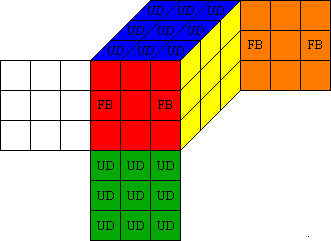
\includegraphics{input/pics/relabel1}
	\caption{\myCaption{A relabeled Rubik's Cube with the up and down faces blue and green respectively, and red and orange as front and back. The grayed facelets are relabeled.}}
	\label{fig:relabel1}
\end{figure}

When relabeling a \rubik{} in the position $s$ it is written as: $r(s)$. A \rubik{} in any position, $s$, is said to be en the set of positions called $H$ if and only if: $r(s)=r(e)$.

The following moves are in the set of moves $A$: U, U', U2, D, D', D2, R2, L2, F2 and B2. If using move sequences in $A$ on a position in $H$, the cube will always be in $H$.


\subsection{First phase}
The first phase of the Kociemba's two phase algorithm takes a scrambled cube $a$ and relabels it $r(a)$ then it finds a move sequence $b$ which will transform the relabeled cube into the subgroup $H$. This move will be denoted: $r(a)\cdot{}b=H$. 
\begin{algorithm}                     
\caption{Kociemba's Algorithm \cite{rokicki09}}          
\label{alg:kociemba}        
\begin{algorithmic}[1]
\STATE $d=0$
\STATE {$l=\infty$}
\WHILE {$d<l$} 
	\FOR {$b \in S^{d}$}
		\IF {$r(ab) \in H$}
			\IF {$d + d_{2}(ab)<l$}
				\STATE Solve phase two, report new better solution
				\STATE {$l=d+d_{2}(ab)$}
			\ENDIF
		\ENDIF
	\ENDFOR
	\STATE {$d=d+1$}
\ENDWHILE
\end{algorithmic}
\end{algorithm}

At first in the algorithm the diameter length ($d$), pictured in figure(somewhere) is set to zero and the length($l$) is set to infinite. The \textbf{while} loop will run as long as $d$ is smaller than $l$. For the first run this i obviously true, and will only test if the scrambled cube already is in the subgroup $H$.

The for loop runs through all move sequences in range $d$. Then an \textbf{if}-statement checks whether the move sequence transforms the cube into the subgroup $H$. $d_2$ is a lookup table which takes a position in $H$ and returns the number of twists it takes to move the postion to $e$ using moves in $A$. If so the algorithm checks whether $d$ + the length of a table lookup, which determine the length of the solution to the position $ab$ is lesser than the length of the last solution. The first time this if statement is run it will return true and this will be the new length of the solution. 

\subsection{Second phase}